
%(BEGIN_QUESTION)
% Copyright 2010, Tony R. Kuphaldt, released under the Creative Commons Attribution License (v 1.0)
% This means you may do almost anything with this work of mine, so long as you give me proper credit

Calculate the voltage sensed by the analog-to-digital converter inside the temperature transmitter:

$$\includegraphics[width=15.5cm]{i00357x01.eps}$$

\underbar{file i00357}
%(END_QUESTION)





%(BEGIN_ANSWER)

Voltage at ADC: {\bf 35.948} millivolts

\vskip 10pt

According to an ITS-90 table for type N thermocouples, the measurement junction will generate 36.577 mV at 1847 $^{o}$F, while the reference junction (at the NX-copper cable junction) will generate 0.629 mV at 75 $^{o}$F.  Since we know these two junctions' voltages are opposed to each other, the voltage seen at the transmitter terminals will be 35.984 mV.

%(END_ANSWER)





%(BEGIN_NOTES)

%INDEX% Measurement, temperature: thermocouple 

%(END_NOTES)

